
\documentclass[a4paper,11pt]{article}
\usepackage[a4paper, margin=8em]{geometry}

% usa i pacchetti per la scrittura in italiano
\usepackage[french,italian]{babel}
\usepackage[T1]{fontenc}
\usepackage[utf8]{inputenc}
\frenchspacing 

% usa i pacchetti per la formattazione matematica
\usepackage{amsmath, amssymb, amsthm, amsfonts}

% usa altri pacchetti
\usepackage{gensymb}
\usepackage{hyperref}
\usepackage{standalone}

% imposta il titolo
\title{Appunti Fondamenti di Automatica}
\author{Luca Seggiani}
\date{2025}

% disegni
\usepackage{pgfplots}
\pgfplotsset{width=10cm,compat=1.9}

% imposta lo stile
% usa helvetica
\usepackage[scaled]{helvet}
% usa palatino
\usepackage{palatino}
% usa un font monospazio guardabile
\usepackage{lmodern}

% tikz in sans
\tikzset{every picture/.style={/utils/exec={\sffamily}}}

\renewcommand{\rmdefault}{ppl}
\renewcommand{\sfdefault}{phv}
\renewcommand{\ttdefault}{lmtt}

% circuiti
\usepackage{circuitikz}
\usetikzlibrary{babel}

% disponi il titolo
\makeatletter
\renewcommand{\maketitle} {
	\begin{center} 
		\begin{minipage}[t]{.8\textwidth}
			\textsf{\huge\bfseries \@title} 
		\end{minipage}%
		\begin{minipage}[t]{.2\textwidth}
			\raggedleft \vspace{-1.65em}
			\textsf{\small \@author} \vfill
			\textsf{\small \@date}
		\end{minipage}
		\par
	\end{center}

	\thispagestyle{empty}
	\pagestyle{fancy}
}
\makeatother

% disponi teoremi
\usepackage{tcolorbox}
\newtcolorbox[auto counter, number within=section]{theorem}[2][]{%
	colback=blue!10, 
	colframe=blue!40!black, 
	sharp corners=northwest,
	fonttitle=\sffamily\bfseries, 
	title=Teorema~\thetcbcounter: #2, 
	#1
}

% disponi definizioni
\newtcolorbox[auto counter, number within=section]{definition}[2][]{%
	colback=red!10,
	colframe=red!40!black,
	sharp corners=northwest,
	fonttitle=\sffamily\bfseries,
	title=Definizione~\thetcbcounter: #2,
	#1
}

% disponi problemi
\newtcolorbox[auto counter, number within=section]{problem}[2][]{%
	colback=green!10,
	colframe=green!40!black,
	sharp corners=northwest,
	fonttitle=\sffamily\bfseries,
	title=Problema~\thetcbcounter: #2,
	#1
}

% disponi codice
\usepackage{listings}
\usepackage[table]{xcolor}

\lstdefinestyle{codestyle}{
		backgroundcolor=\color{black!5}, 
		commentstyle=\color{codegreen},
		keywordstyle=\bfseries\color{magenta},
		numberstyle=\sffamily\tiny\color{black!60},
		stringstyle=\color{green!50!black},
		basicstyle=\ttfamily\footnotesize,
		breakatwhitespace=false,         
		breaklines=true,                 
		captionpos=b,                    
		keepspaces=true,                 
		numbers=left,                    
		numbersep=5pt,                  
		showspaces=false,                
		showstringspaces=false,
		showtabs=false,                  
		tabsize=2
}

\lstdefinestyle{shellstyle}{
		backgroundcolor=\color{black!5}, 
		basicstyle=\ttfamily\footnotesize\color{black}, 
		commentstyle=\color{black}, 
		keywordstyle=\color{black},
		numberstyle=\color{black!5},
		stringstyle=\color{black}, 
		showspaces=false,
		showstringspaces=false, 
		showtabs=false, 
		tabsize=2, 
		numbers=none, 
		breaklines=true
}

\lstdefinelanguage{javascript}{
	keywords={typeof, new, true, false, catch, function, return, null, catch, switch, var, if, in, while, do, else, case, break},
	keywordstyle=\color{blue}\bfseries,
	ndkeywords={class, export, boolean, throw, implements, import, this},
	ndkeywordstyle=\color{darkgray}\bfseries,
	identifierstyle=\color{black},
	sensitive=false,
	comment=[l]{//},
	morecomment=[s]{/*}{*/},
	commentstyle=\color{purple}\ttfamily,
	stringstyle=\color{red}\ttfamily,
	morestring=[b]',
	morestring=[b]"
}

% disponi sezioni
\usepackage{titlesec}

\titleformat{\section}
	{\sffamily\Large\bfseries} 
	{\thesection}{1em}{} 
\titleformat{\subsection}
	{\sffamily\large\bfseries}   
	{\thesubsection}{1em}{} 
\titleformat{\subsubsection}
	{\sffamily\normalsize\bfseries} 
	{\thesubsubsection}{1em}{}

% disponi alberi
\usepackage{forest}

\forestset{
	rectstyle/.style={
		for tree={rectangle,draw,font=\large\sffamily}
	},
	roundstyle/.style={
		for tree={circle,draw,font=\large}
	}
}

% disponi algoritmi
\usepackage{algorithm}
\usepackage{algorithmic}
\makeatletter
\renewcommand{\ALG@name}{Algoritmo}
\makeatother

% disponi numeri di pagina
\usepackage{fancyhdr}
\fancyhf{} 
\fancyfoot[L]{\sffamily{\thepage}}

\makeatletter
\fancyhead[L]{\raisebox{1ex}[0pt][0pt]{\sffamily{\@title \ \@date}}} 
\fancyhead[R]{\raisebox{1ex}[0pt][0pt]{\sffamily{\@author}}}
\makeatother

\begin{document}

% sezione (data)
\section{Lezione del 07-05-25}

% stili pagina
\thispagestyle{empty}
\pagestyle{fancy}

% testo
\subsection{Margini di ampiezza e fase}
Vogliamo adesso valutare la \textbf{robustezza} dei sistemi, cioè quantificare la stabilità di un sistema in ciclo chiuso conoscendone la risposta armonica in catena aperta.

Il sistema considerato sarà sempre lo stesso, con funzione di trasferimento in catena chiusa $W(s)$:
$$
W(s) = \frac{Y(s)}{R(s)} = \frac{K \cdot G(s)}{1 + K \cdot G(s)} = \frac{\hat{G}(s)}{1 + \hat{G}(s)}
$$
dove le lettere vengono cambiate ad arbitrio fra un esempio e l'altro per vedere se il lettore sta attento.

Prendiamo ad esempio la funzione di trasferimento in catena aperta $G(s)$:
$$
G(s) = \frac{1}{s (s + 1)^2}
$$
e tracciamone il luogo delle radici:
\begin{center}
	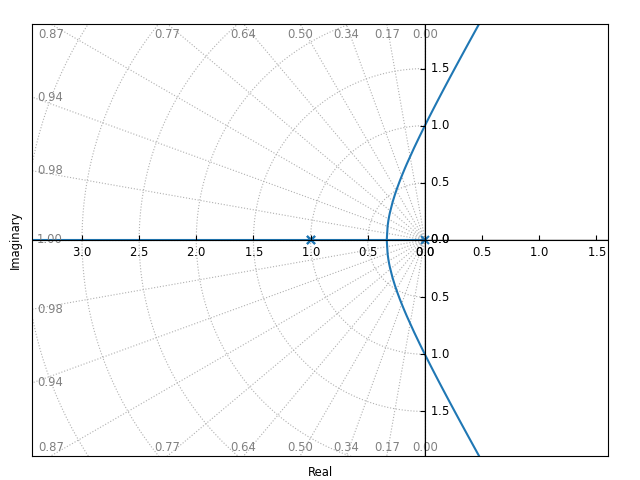
\includegraphics[scale=0.7]{../figures/rlocus_margin.png}
\end{center}
da cui notiamo che 2 poli si dividono a circa $-\frac{1}{2}$ nei rami all'infinito, che per un certo valore di $K$ intersecano l'asse immaginario, e quindi passano nella parte di piano $\mathrm{Re} > 0$. 

Sappiamo che questo è il punto $K_{crit}$ dove il sistema diventa instabile.
Vediamo che questo valore è $K_{crit} = 2$.

\subsubsection{Margini di ampiezza e fase su Bode}

Tracciamo quindi il diagramma di Bode per $K = K_{crit}$, cioè:
$$
G(s) = \frac{2}{s(s + 1)^2}
$$
questo avrà il seguente aspetto:
\begin{center}
	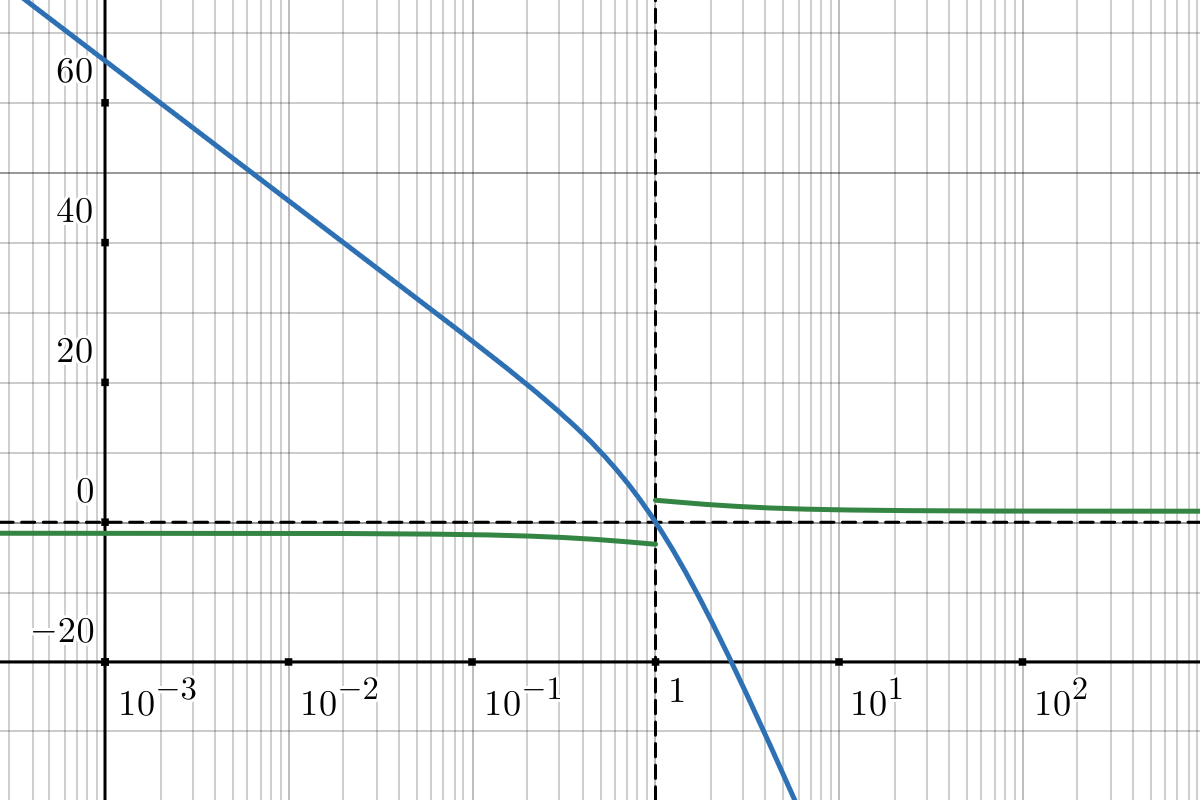
\includegraphics[scale=0.8]{../figures/bode_margin.png}
\end{center}

Tracciando il diagramma di Bode, notiamo che con $K = K_{crit}$:
\begin{itemize}
	\item La fase deve essere maggiore di $-180^\circ$ quando il diagramma di modulo è maggiore di 0 dB;
	\item La fase deve essere minore di $-180^\circ$ quando il diagramma di modulo è minore di 0 dB;
\end{itemize}
cioè fondamentalmente:
\begin{itemize}
	\item La fase deve $-180^\circ$ nel punto in cui il diagramma del modulo passa per il punto di crossover a 0 dB.
\end{itemize}

Vedremo poi che questa non è altro che la condizione del criterio di Nyquist relativa al punto $-1$.

Introduciamo quindi due misure dette:
\begin{itemize}
	\item \textbf{Margine di fase}:
		$$
			M_\Phi = 180^\circ + \Phi(\omega_t)
		$$
		cioè l'angolo che si ricava dalla somma di $180^\circ$ più la fase della funzione di trasferimento ad anello aperto alla pulsazione di crossover a 0 dB.

		Chiaramente il margine di fase è vantaggioso quando è $> 0$, in quanto significa che $K < K_{crit}$  quindi il sistema è stabile.
	\item \textbf{Margine di ampiezza}, o \textit{margine di guadagno}:
		$$
			M_{g_{dB}} = 0 - |G(s)|_{dB} \big|_{\Phi = - \pi}
		$$
		cioè la differenza fra 0 e il valore in dB del modulo della $G(s)$ quando la fase della $G(s)$ ad anello aperto vale $-180^\circ$.

		Per convenzione si ha che:
		\begin{itemize}
			\item $M_g$ è \textit{positivo} se $|G(s)|$ è al di sotto di 0 dB per fase $-180^\circ$, cioè il sistema è \textbf{stabile};
			\item $M_g$ è \textit{negativo} se $|G(s)$ è al di sopra di 0 dB per fase $-180^\circ$, cioè il sistema è \textbf{instabile}.
		\end{itemize}

	In particolare, il margine di guadagno rappresenta quanto è possibile aumentare il guadagno del sistema prima di raggiungere l'instabilità.

	Notiamo poi che esiste una definizione alternativa di margine di ampiezza, utile nell'analisi dei margini di fase sul diagramma di Nyquist (che vedremo fra poco), che è:
	$$
	M_g = -\frac{1}{|G(s)|} \Bigg|_{\phi = -\pi}
	$$
\end{itemize}

Vediamo quindi un grafico che evidenzia, per il sistema appena considerato, a guadagno unitario, il margine di guadagno e di fase:

\begin{center}
	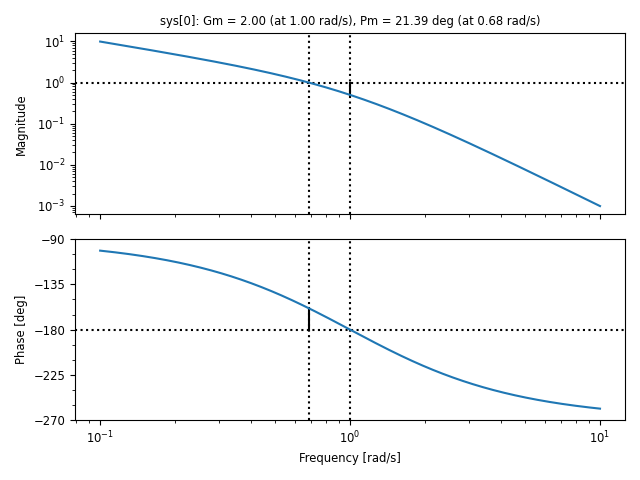
\includegraphics[scale=0.8]{../figures/margins.png}
\end{center}

Notiamo che il grafico, generato con la libreria \href{https://github.com/python-control/python-control}{Control} di Python, riporta anche i margini di guadagno (\textsf{Gm}) e di fase (\textsf{Pm}), coi relativi punti di valutazione (cioè rispettivamente i punti di crossover a $-180^\circ$ e $0 dB$).

Di questi, notiamo che il margine di guadagno è espresso nella seconda modalità che abbiamo riportato, cioè come:
$$
G_m = \frac{1}{|G(j \omega_\text{crossover})|}
$$

Infatti avremo che per il punto di crossover a $-180^\circ$, che si trova a 1 rad/s, il modulo vale circa $-6 \, \mathrm{dB}$, che sappiamo corrispondere a $\frac{1}{2}$, per cui:
$$
G_m = \frac{1}{\frac{1}{2}} = 2
$$

\subsubsection{Margini di ampiezza e fase su Nyquist}
La definizione di margini di fase e ampiezza richiede una qualche constatazione sul diagramma di Nyquist, che sappiamo esprimere le stesse informazioni del diagramma di Bode.

Sul diagramma di Nyquist considereremo quindi il punto a 0 dB con fase $-180^\circ$, cioè il punto -1.

Vediamo ad esempio la funzione di trasferimento vista prima tracciata con Nyquist:
\begin{center}
	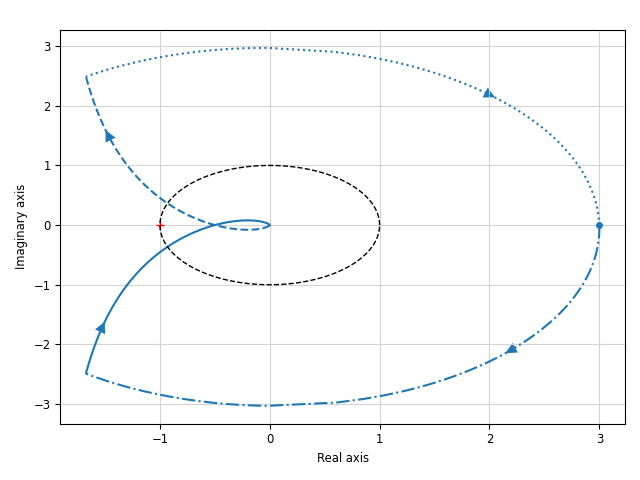
\includegraphics[scale=0.8]{../figures/nyquist_margin.png}
\end{center}

In questo caso il margine di \textbf{fase} sarà dato dall'angolo $\phi_m$ che il punto di passaggio del diagramma di Nyquist per la circonferenza di raggio unitario forma con $-1$ (che è stata tracciata in nero nel grafico).

Il margine di \textbf{guadagno} $\omega_\pi$ sarà invece la distanza del punto del diagramma di Nyquist con fase $-180^\circ$ dal punto critico $-1$.

Da qui la seconda definizione che abbiamo dato di margine di guadagno: preso $\omega_\pi = |G(j \omega)| \big|_{\Phi = -\pi}$, abbiamo che questo passa per il punto critico $-\frac{1}{K}$ quando:
$$
\omega_\pi = |G(j\omega_\Phi)| = 1 
$$
e quindi potrà interessarci il rapporto:
$$
G_M = \frac{1}{|G(j\omega_\Phi)|}
$$
che possiamo intendere come la costante moltiplicativa massima che possiamo applicare al guadagno prima di rendere il sistema instabile.

\subsubsection{Specifiche generali per i margini}

Abbiamo quindi visto il significato nei diagrammi di Bode e Nyquist dei margini di fase e guadagno.
Abbiamo che in casi reali si hanno buone condizioni di stabilità con:
\begin{itemize}
	\item Margine di fase: $M_G > 4 - 6 dB$, cioè si può circa raddoppiare il gaudagno;
	\item Margine di fase: $M_F > \sim 35^\circ$.
\end{itemize}

\subsubsection{Margini per sistemi irregolari}
Inoltre, notiamo che le definizioni che abbiamo visto sono \textit{ben strutturate} solo per i cosiddetti sistemi \textbf{regolari}, mentre sono poco significative per sistemi non regolari.

Definiamo quindi il significato di sistema regolare:
\begin{definition}{Sistema regolare}
	Un sistema in retroazione ha un andamento regolare se l'ampiezza della funzione di trasferimento a ciclo aperto è una funzione monotona decrescente della pulsazione.
\end{definition}

Questo significa essenzialmente che quando si hanno più intersezioni con l'asse a 0 dB su Bode, o con la circonferenza unitaria su Nyquist, la definizione di margine di fase o ampiezza perde l'univocità.
In questi casi, chiaramente, vorremo considerare il caso peggiore e quindi i margini più piccoli, cioè più vicini a portare all'instabilità.

\par\medskip

Una nota va fatta anche su sistemi che risultano instabili a bassi guadagni, e diventano stabili all'aumentare di $K$.
In questo caso, infatti, dovremo in qualche modo invertire la definizione dei margini.

Prendiamo ad esempio la funzione di trasferimento:
$$
G(s) = \frac{\left(1 + \frac{s}{10}\right)^2}{s^2 (s + 1)}
$$

\noindent

\begin{minipage}{\textwidth}

In questo caso i margini sul diagramma di Bode avranno il seguente aspetto:
\begin{center}
	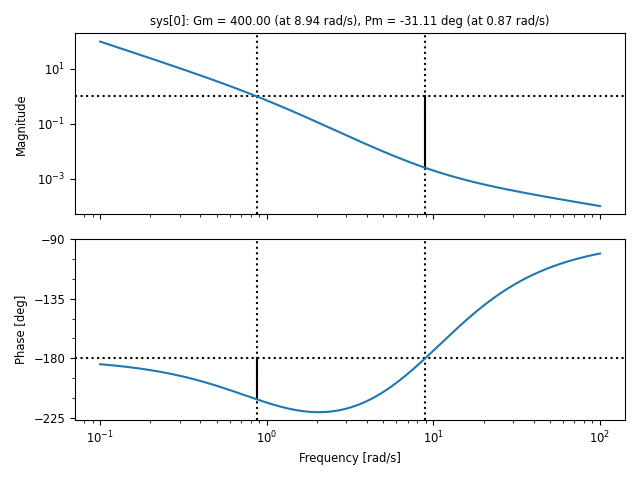
\includegraphics[scale=0.75]{../figures/bode_margin_weird.png}
\end{center}

\end{minipage}

da dove notiamo che il margine di fase a $0.87$ rad/s è negativo, cioè il sistema è instabile.

Accorgiamoci quindi di poter aumentare il guadagno fino a 400 (il margine di guadagno), per cui si ottiene la funzione di trasferimento:
$$
K \cdot  G(s) = 400 \frac{\left(1 + \frac{s}{10}\right)^2}{s^2 (s + 1)}
$$
e i margini:
\begin{center}
	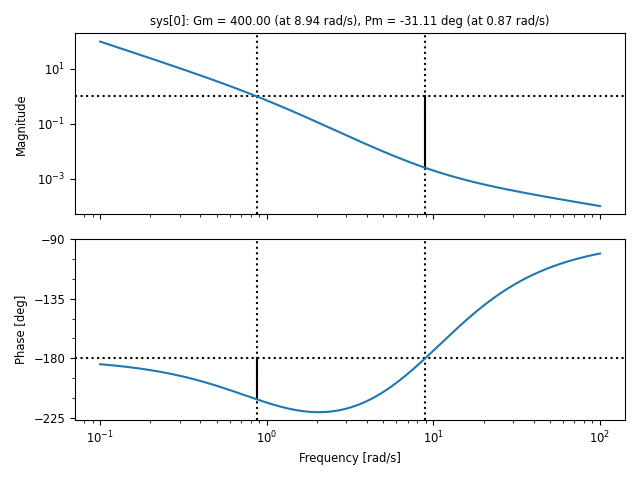
\includegraphics[scale=0.75]{../figures/bode_margin_weird.png}
\end{center}
da dove notiamo che siamo riusciti ad annullare entrambi i margini.

Una spiegazione alternativa per il valore di guadagno 400 si può avere anche attraverso il luogo delle radici:
\begin{center}
	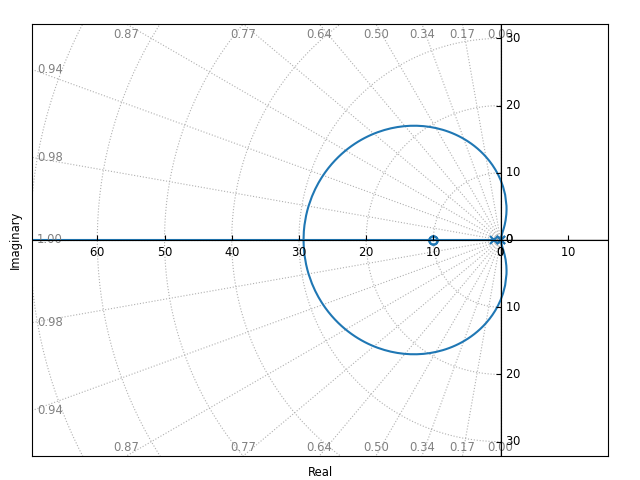
\includegraphics[scale=0.8]{../figures/weird_margin_rlocus.png}
\end{center}
per cui si nota che nel luogo diretto, fino a un certo valore di $K$ si hanno i poli positivi sui rami che escono dall'asse reale.
Il $K$ critico di 400 sarà proprio quel guadagno necessario a tornare nella parte negativa del piano, e quindi alle condizioni di stabilità.

\subsection{Sistemi di controllo}
Veniamo quindi alla fase di progetto vera e propria del controllore $C(s)$ insrito nella catena di retroazione.
Per fare cioò modifichiamo lo schema in catena chiusa come segue:
\begin{center}
	\begin{tikzpicture}
		\draw (1,0) rectangle (3, 1);
		\node at (2, 0.5) {$G(s)$};

		\draw (-3,0) rectangle (-1, 1);
		\node at (-2, 0.5) {$C(s)$};

		\draw[-stealth] (-7, 0.5) -> (-5.1, 0.5);
		\draw[-stealth] (-5, 0.5) -> (-3, 0.5);
		\draw[-stealth] (-1, 0.5) -> (1, 0.5);
		\draw[-stealth] (3, 0.5) -> (7, 0.5);

		\draw (5, 0.5) -> (5, -2);
		\draw (5, -2) -> (-5, -2);
		\draw[-stealth] (-5, -2) -> (-5, 0.4);

		\draw[fill=white] (-5, 0.5) circle (0.1);

		\node at (-6, 0.75) {$R(s)$};
		\node at (6, 0.75) {$Y(s)$};

		\node at (-4.75, 0.75) {$+$};
		\node at (-4.75, 0.25) {$-$};

		\node at (0, 0.75) {$U(s)$};
		\node at (-3.8, 0.75) {$E(s)$};
	\end{tikzpicture}
\end{center}

# mancano disturbi e variabili controllate

Dove:
\begin{itemize}
	\item $R(s)$ è il riferimento;
	\item $E(s)$ è l'errore;
	\item $U(s)$ è la variabile di controllo (manipolabile);
	\item $D(s)$ sono i disturbi (non manipolabili);
	\item $Y(s)$ è l'uscita, quindi le variabili misurate;
	\item $Z$ sono le variabili controllate, non necessariamente misurate.
\end{itemize}

Vorremo quindi sviluppare un controllore che non assicura più solo la stabilità del sistema, ma anche:
\begin{itemize}
	\item Adeguata precisione, sopratutto in termini di errore a regime;
	\item Adeguata stabilità, in termini di incertezza e margini.
\end{itemize}

\subsubsection{Trasferimento del sensore}
Facciamo un commento sull'eventuale sensore $H(s)$.
# diagramma modificato con $H(s)$

In questo caso la funzione di trasferimento in catena chiusa, che avevamo con $H(s) = 1$ essere:
$$
W(s) = \frac{C(s) G(s)}{1 + C(s) G(s)}
$$
cambierà diventando:
$$
W'(s) = \frac{C(s) G(s)}{1 + C(s) G(s) H(s)} = \frac{1}{H(s)} \cdot \frac{C(s) G(s) H(s)}{1 + C(s) G(s) H(s)}
$$
cioè si potra considerare la stessa forma:
$$
\frac{C(s) G(s) H(s)}{1 + C(s) G(s) H(s)} \sim \frac{\hat{G}(s)}{1 + \hat{G}(s)}
$$
a cui siamo abituati, e applicare quanto studiato finora sullo studio dei sistemi in catena chiusa dalla funzione di trasferimento in catena aperta.

Decideremo quindi di trascurare il sensore finora, consci di non ledere alla generalità della trattazione in quanto andrà semplicemente aggiunto alla funzione di trasferimento in catena aperta.

\subsubsection{Disturbi e specifiche}
Vediamo quindi che le performance che desideriamo in ciclo chiuso sono:
\begin{itemize}
	\item Il sistema in ciclo chiuso deve essere \textbf{stabile};
	\item Il sistema in ciclo chiuso deve inseguire i riferimenti, e la risposta deve essere \textbf{rapida} e "liscia" rispetto a variazioni nei riferimenti (\textit{set-point tracking});
	\item Il sistema deve \textbf{reiettare i disturbi}: gli effetti dei disturbi sul sistema devono essere minimizzati.
\end{itemize}

Definiamo quindi i seguenti tipi di specifiche:
\begin{itemize}
	\item Specifiche \textbf{statiche}, riguardanti il comportamento a regime di un sistema controllato e quindi comprendenti la scelta di un controllore in grado di annullare o ridurre l'errore in risposta a un riferimento o a un segnale di disturbo. Chiamiamo \textbf{errore a regime} l'errore su un'orizzonte temporale teoricamente infinito;
	\item Specifiche \textbf{dinamiche}: riguardanti tempo di risposta, smorzamento, ecc...;
	\item Specifiche di \textbf{robustezza}, essenzialmente i margini di guadagno e di fase;
\end{itemize}

\subsubsection{Disturbi interni}
Possiamo estendere la trattazione dei disturbi a diversi tipi di \textit{disturbi interni}:
\begin{itemize}
	\item \textbf{Disturbo interno al controllore:} possiamo immaginare che ci sia un disturbo che si va ad inserire fra il controllore $C(s)$ e il sistema $G(s)$.
		
		# diagramma

	\item \textbf{Disturbo interno al sistema:} possiamo avere un sistema diviso in più sottosistemi, poniamo $G_1(s)$ e $G_s(2)$, e un disturbo interno posto fra i due.
		
		# diagramma

		In questo caso la funzione di uscita avrà una forma del tipo:
		$$
		Y(s) = W(s) \cdot R(s) + W_d(s) \cdot D(s)
		$$
		con:
		$$
		W(s) = \frac{C(s) G_1(s) G_2(s)}{1 + C(s) G_1(s) G_2(s)}, \quad W_d(s) = \frac{G_2(s)}{1 + C(s) G_1(s) G_2(s)}
		$$
		direttamente dalla combinazione degli effetti della retroazione su $W(s)$ e del disturbo interno sulla sola parte $W_d(s)$ (quella di $G_2(s)$, che sta a valle del disturbo $D(s)$).
		
\end{itemize}
\end{document}
